\chapter{Setup}
In this chapter we explain the setting up of RTDS model and the code for observability analysis and state estimation

%Replace \lipsum with text.
% You may have as many sections as you please. This is just for reference.

\section{RTDS}
RTDS \cite{rtds} is a popular simulation hardware used to run real time power line simulations. It is commonly  used for studies of protective relays, control systems, power hardwares, etc. We use this hardware primarily to simulate a Transmission line and generate and record data for further analysis, such as observability analysis, state estimation, Optimum Power Flow, etc.\\
RSCAD is a simulation software that is used to create models of power lines, to work on the RTDS Simulator Hardware. For our project we set up a model for a 14 bus power line system, with specifications taken from IEEE 14 Bus power system \cite{IEEE14bus}. The model has the following characteristics:
\begin{itemize}
\item Number of Buses: 14
\item Number of Lines: 20
\item Number of Generators: 5
\end {itemize}
The overall system that we designed looked like Figure ~\ref{fig:ckt}.\\
\begin{figure}[h]
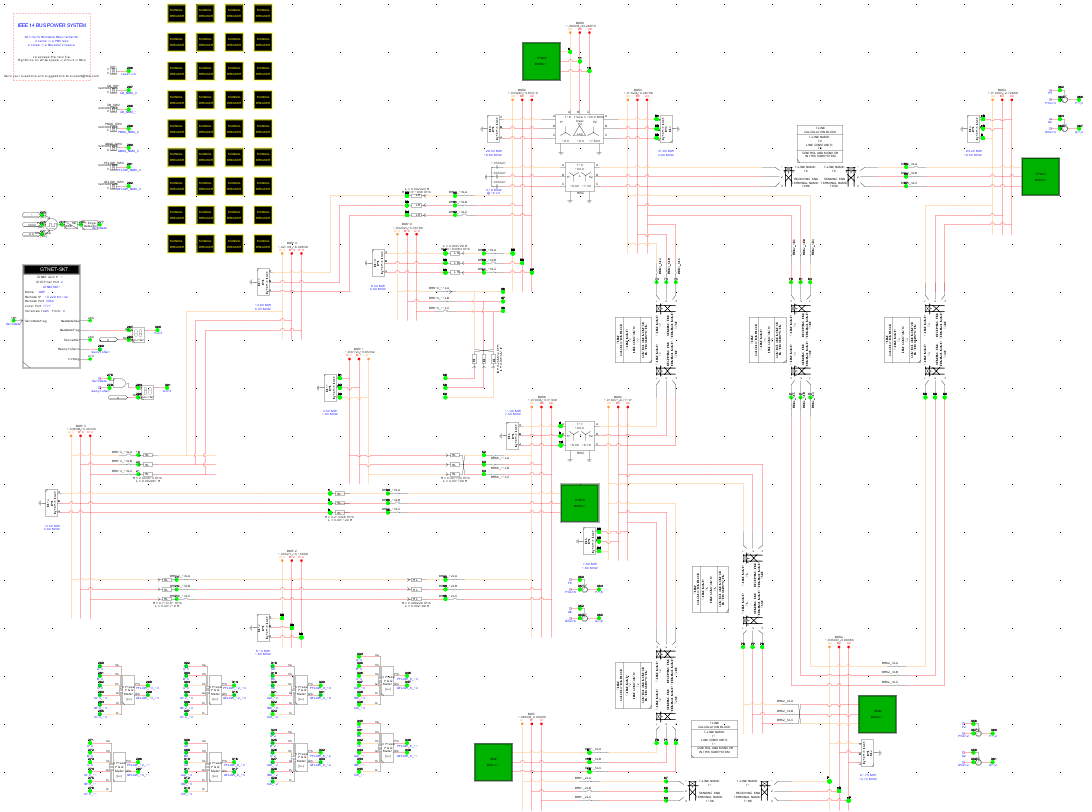
\includegraphics[width=\textwidth]{Figures/ckt.png}
\caption{IEEE 14 Bus Power Line System Model on RSCAD}\label{fig:ckt}
\end{figure}

It had the following key blocks, shown here for reference. (~\ref{fig:bus} to ~\ref{fig:skt})

\begin{figure}[h]
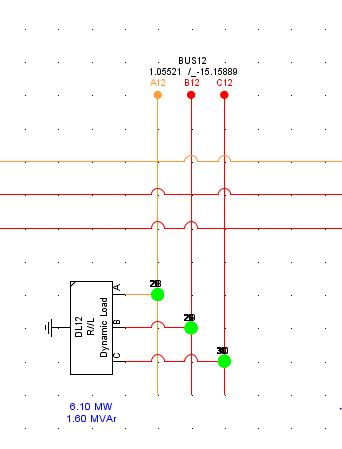
\includegraphics[width=\textwidth]{Figures/bus.jpg}
\caption{Typical Bus in RSCAD}\label{fig:bus}
\end{figure}

\begin{figure}[h]
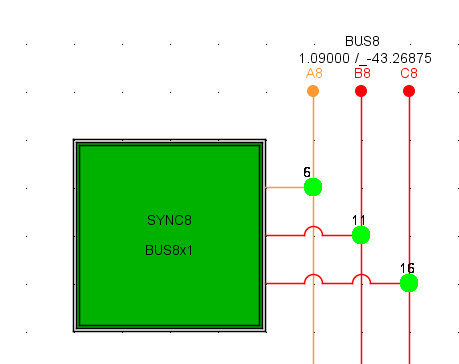
\includegraphics[width=\textwidth]{Figures/gen.png}
\caption{Generator Block in RSCAD}\label{fig:gen}
\end{figure}

\begin{figure}[h]
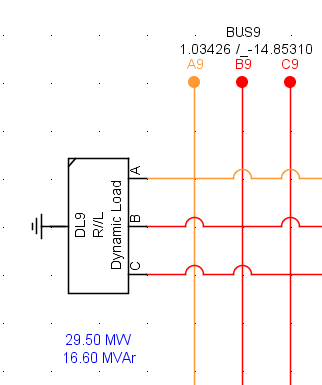
\includegraphics[width=\textwidth]{Figures/load.png}
\caption{PQ load Block in RSCAD}\label{fig:load}
\end{figure}

Apart from the main network, we have the GTNET-SKT block ( Figure ~\ref{fig:skt}), which is crucial for sending and receiving data from RTDS to our server, which records and processes data for further analysis of the power system.  To function, it needs the following parameters specified:
\begin{itemize}
\item All the signals to be measured. In our case, these were the status about all the circuit breakers in the system, the real and complex power injections, real and complex power flows in the lines, and status about availability of each measurement
\item The remote IP address and port of the server to which data is to be sent. 
\end{itemize}
GTNET-SKT sends raw data over UDP protocol to the server, and each measurement is just a 32 bit Floating point number or a 32 bit signed Integer. 
It further places a restriction, that we can send only upto 300 measurements per GTNET-SKT block. For more measurements, we add more blocks, and server will then have to communicate with RTDS over multiple ports, which would become complicated as more blocks are added. 
Furthermore, in real life situations, not all data measurements are available, so we also need to check which measurements correspond to which variables. We simulate this condition by toggling the availability of measurements recorded by GTNET-SKT. 
With all this in mind, we see that while the essential information about which measurement corresponds to which variable is critical, we can not simply transmit the measurement labels with each measurement since we would be essentially doubling the number of variables used for transmission of same number of measurement values.\\
To counter these points, we developed an efficient scheme to transmit information about labels over GTNET-SKT.
\\Firstly, we figured that all the topological information about a network (the number of buses, number and connectivity of lines, generator buses etc.), as well as information about the line impedances remain fixed, and that information can be stored in files we will call \emph{casefiles}, since most networks used for power line research are typically standard networks, described in IEEE standards. MATPOWER, a MATLAB based application for calculating load flow of power systems, and PyPower, it's python equivalent, typically work on these standard configurations, and they store the above information about a network in casefiles, in a similar fashion to what we are doing. Specifying the casefile will tell us everything we need to know about the topology of the network, it's number of buses, lines, and circuit breakers, as well as the total real and reactive power injection and flow measurements.\\
To allow the flexibility to work with a non-standard network configuration, we gave the user an option to create it's own casefile, and we would then use their custom casefiles to process topological information about their network instead. 
\\Second, we created an order in which the measurements from the GTNET-SKT will be transmitted. We will first send all the circuit breaker information, then the real power injections at the buses, then the reactive power injections, then real power line flows, and then reactive power line flows. The order of transmitting data about buses follows the following rule:
\begin{itemize}
\item \emph{For two buses with bus numbered \textbf{a} and \textbf{b}, measurement related to bus \textbf{a} will come before bus \textbf{b} if $\textbf{a}<\textbf{b}$}
\end{itemize}
For measurements related to lines, we follow the following rule:\\
\emph{Information about a line between buses numbered \textbf{a} and \textbf{b} (where $\textbf{a}<\textbf{b}$), will come before information about a line between buses numbered \textbf{c} and \textbf{d} (where $\textbf{c}<\textbf{d}$) if: $$\textbf{a} < \textbf{c}, \textrm{ or } (\textbf{a}=\textbf{c} \textrm{ and }  \textbf{b}<\textbf{d})$$}

Thirdly, we reasoned that status of availability of each measurement can be encoded in 1 bit each. Therefore, for maximum of \emph{n} possible measurements needed, we will need exactly \emph{n} bits, or approx \emph{n/32} measurement variables to tell whether each measurement is available or not. Coupled with the ordering in which each measurement comes from RTDS, this allows us to know exactly which information is coming, without explicitly sending the labels!\\
We will call these \emph{n/32} measurement variables as \textbf{status numbers}, since they provide us information about availability status of each measurement. \\
The order in which RTDS sends information about the system:
\begin{itemize}
\item \textbf{case\_number}, informing us about the topology of the network
\item \textbf{status number} about the availability of circuit breaker measurements,
\item \textbf{Circuit breaker measurements} 
\item \textbf{status number} about the availability of real power injections
\item \textbf{Real power injection measurements} 
\item \textbf{status number} about the availability of reactive power injections
\\ \textbf{\dots}
\item \textbf{status number} about the availability of reactive power flows
\item \textbf{Reactive power flow measurements} 
\end{itemize}

\begin{figure}[h]
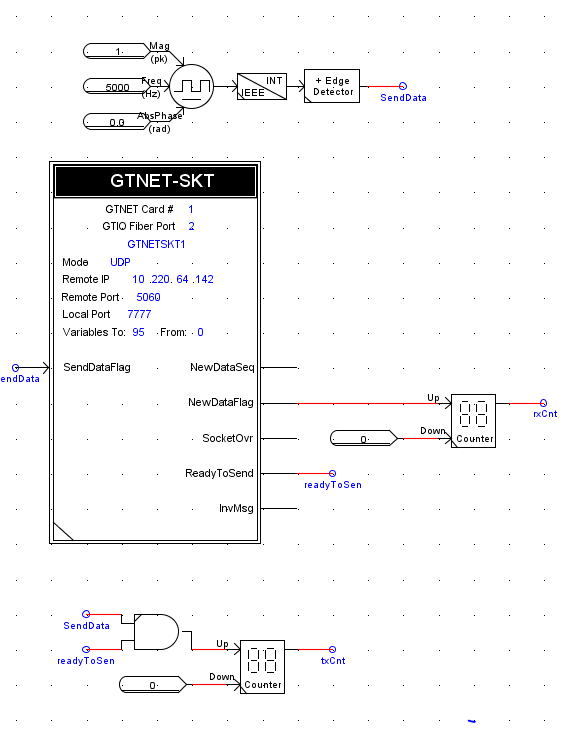
\includegraphics[width=\textwidth]{Figures/skt.png}
\caption{GTNET-SKT Block in RSCAD}\label{fig:skt}
\end{figure}



\section{Server side data receiving and processing}
We provide a remote IP address and port number to GTNET-SKT, which is the address at which our server is listening to receive the packets of data from RTDS. We wrote a Python Script to act as the server and receive data. This script is present in the Appendix.\\
Since RTDS just sends packets with 32 bit blocks for each measurement, we need to process the binary message packet to obtain meaningful information. To decode this information, we also need to remember that the information can either be a Floating point value, or an Integer. We had to observe and figure out the fact that for floating point numbers, the GTNET-SKT encodes it in IEEE 754 standard for 32 bit Floating point format, which is that the MSB is the sign bit, then the next 8 bits are for the exponent, and the rest 23 bits are for the mantissa. To get the floating point number from a 32 bit binary string, as given by IEEE 754 standards:
\begin{itemize}
\item Let e= decimal value of exponent part of the string
\item For base, we note that mantissa represents the fractional part of the number. Say, for example mantissa is given by $0111001\dots$, then the number, in binary form will be given by $1.0111001\dots$ Base is the decimal value of this number
\item Finally, the floating point number f=base$\cdot2^{(e-127)}$
\end{itemize}
If, however, the measurement is an integer value, a simple binary to decimal conversion of that 32 bit binary number will give us the result. We use the integer values mainly for the status number measurements, since encoding the status of each measurement will involve encoding the binary string into an integer number or a float, and the former one is much much easier to do, and much easier to implement for a user on RTDS side, since that is where the status number will come from.
Thus, given our expectation of data type of each measurement, we can appropriately decode the binary data into real valued measurements about active and reactive power.
\section{Casefiles}
MATPOWER, and by extension, PyPower provides us the casefiles for a lot of different IEEE standard transmission line systems, ranging from 6-bus or 9-bus system to 300 bus systems. If we know the casefile for the system at hand, we can decode the topological information about the system, as well as get useful information like line impedances, and generation costs defined for the generators in the system. Decoding the data received from RTDS, we learn the case\_number of the system from the first measurement, and we can use this to get the appropriate case file.
All case files contain the following data:
\begin{itemize}
\item \textbf{Bus Data:} For each bus in the system, tells us about its type (PV,PQ or Slack), baseKV rating, voltage limits, real and reactive power loads at that bus, etc.
\item \textbf{Line/Branch Data:} For each line/branch, it tells us about the buses it is connected to, its impedances, status, etc.
\item \textbf{Generator Data:} Tells us which bus each generator is connected to, it's real and reactive power generation, terminal voltage, reactive power limits, AGC participation factors, etc.
\item \textbf{Generation Cost Data:} For each generator, it has the coefficients \emph{(a,b,c)} of generation cost as a function of real power generated ($Cost=a\cdot P^2+b\cdot P+c$), and the time it stays shut down.
\end{itemize}
\section{Observability Analysis}

\section{State Estimation}
